\documentclass[a4paper]{article}
\usepackage{interspeech2012,amssymb,amsmath,graphicx}
\sloppy	% better line breaks
%\ninept	% optional

\title{Identifying Speakers' Personal Information in Phone Conversations}

%%%%%%%%%%%%%%%%%%%%%%%%%%%%%%%%%%%%%%%%
%% If multiple authors, uncomment and edit the lines shown below.       %%
%% Note that each line must be emphasized {\em } by itself.                  %%
%% (by Stephen Martucci, author of spconf.sty).                                     %%
%%%%%%%%%%%%%%%%%%%%%%%%%%%%%%%%%%%%%%%%
%\makeatletter
%\def\name#1{\gdef\@name{#1\\}}
%\makeatother
%\name{{\em Firstname1 Lastname1, Firstname2 Lastname2, Firstname3 Lastname3,}\\
%      {\em Firstname4 Lastname4, Firstname5 Lastname5, Firstname6 Lastname6,
%      Firstname7 Lastname7}}
% End of required multiple authors changes %%%%%%%%%%%%%%%%%

\makeatletter
\def\name#1{\gdef\@name{#1\\}}
\makeatother
\name{{\em Shi Hu, Peter Lipay}}

\address{Stanford University \\
{\small \tt \{s3hu and plipay\}@cs.stanford.edu}}

%\twoauthors{Karen Sp\"{a}rck Jones.}{Department of Speech and Hearing \\
%  Brittania University, Ambridge, Voiceland \\
%  {\small \tt Karen@sh.brittania.edu} }
%  {Rose Tyler}{Department of Linguistics \\
%  University of Speechcity, Speechland \\
%  {\small \tt RTyler@ling.speech.edu} }

\begin{document}
\maketitle


\begin{abstract}
In this report, we investigate various methods to estimate a speaker's background information using their phone conversations and the corresponding transcripts. Among other results, we achieved 98\% estimation accuracy in gender, and 68\% in education level using speech data alone. This report also includes the most discriminative words for gender derived from the KL distance, and a simulation of a speech recognition system to show the robustness of our methods using the ``transcribed'' text.
\end{abstract}


\section{Introduction}
Being able to automatically identify a speaker's background information in a phone conversation can have many benefits. For example, when a human interacts with a conversational agent, knowing the person's age can help machines customize their responses. Other usages may include targeted advertising and criminal investigation. In this report, we estimate a speaker's age, gender, education level and American English accent using their speech and transcripts in phone conversations.

\section{Related Work}
Bahari et al. extracted speech patterns based on i-vectors \cite{dehak}, then apply Support Vector Regression (SVR) to estimate the age of speakers \cite{bahari}. An i-vector or identity vector is a low-dimensional representation of a speaker obtained by projecting the speaker utterance onto the total variability space, which contains both speaker and channel variability (the basis is denoted as T in equation \ref{ivector}).  The speaker- and channel-dependent GMM mean supervector $\mu$ is modeled as:  
\begin{equation}
\mu = m + Tw
\label{ivector}
\end{equation}

Here, $m$ is the speaker- and channel-independent mean supervector. The i-vector is represented as $w$.

Bahari et al. used a 60 dimensional feature vector consisting of 20 MFCCs appended by their derivatives to train the GMM system, and used a variation of $\mu$ and $m$ to obtain the i-vector. They showed that the age is best estimated without any dimension reduction on the i-vector, and the mean absolute error (MAE) in years for male and female speakers' age is 7.63 and 7.61, respectively.

Garera and Yarowsky discussed several techniques to classify gender, age, etc using text only \cite{garera}. They used unigrams and bigrams with top tf-idf scores and stopwords as the features, and a linear SVM classifier for training and testing. For gender/age detection, they found the partner of a conversation has strong influence on the choice of words on both sides. Thus, they classify both partners jointly, e.g., male-male vs rest or female-female vs rest, and achieved better accuracy than classifying each partner separately. In addition, they found sociolinguistic features such as speaker rate and pronoun usage are good indicators of gender, etc.

Boulis and Ostendorf analyzed the differences in word use between genders using phone conversation transcripts \cite{boulis}. To obtain the best classification accuracy of conversation sides according to the genders, they used the top 70\% of all bigrams in the corpus as features, sorted by the KL distance, the tf-idf as the feature scores and SVM as the classifier. This achieved an accuracy of around 93\%. However, using only 3\% of the top bigrams can still achieve around 90\% accuracy. Further, they found the conversation partners influence each other's linguistic patterns; hence, it is easier to classify same-gender conversations than cross-gender. 

\section{Methods}

\subsection{Datasets}
We are using the Switchboard Phase 2 corpus which was recorded in 1991/2. There are 543 speakers and 2262 phone conversations, consisting of 243 hours of speaking time, and 2.9M spoken words. We want to separate out the two speakers in each conversation. For audio files, we used sox to extract the conversation side for each speaker, and concatenate all segments together. For text files, we extract and concatenate the utterences by speakers.

As for the speaker properties, there are 2 genders, 5 education levels, 10 American English accents and 6 age groups (grouped by decades). Their distributions are plotted in Figure \ref{dists}. For age, we also used regression to compute mean absolute error (MAE) using chronological age.

\begin{figure}[t]
\centerline{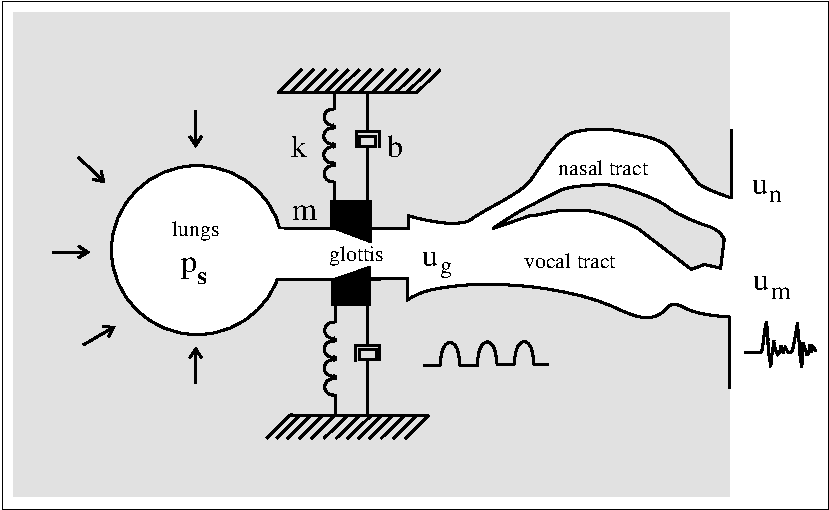
\includegraphics[width=80mm]{figure}}
\caption{{\it Speaker property distributions}}  
\label{dists}
\end{figure}

\begin{itemize}
%\itemsep -1.3mm
\item Proceedings will be created in A4 paper size.
Authors must therefore submit their papers in A4 paper size.
\item Two columns are used except for the title part and possibly for large 
figures that need a full page width.
\item Left margin is 20 mm.
\item Column width is 80 mm.
\item Spacing between columns is 10 mm.
\item Top margin 25 mm (except for the first page which is 30 mm to the title top).
\item Text height (without headers and footers) is maximum 235 mm.
\item Headers and footers must be left empty.
The conference publication company will add information for publication.
\item Check indentations and spacings by comparing to this 
example file (in PDF).
\end{itemize}


\subsubsection{Headings}
Section headings are centered in boldface with the first word capitalized and the rest of the heading in lower case.
Sub-headings appear like major headings, except they start at the left margin in the column.
Sub-sub-headings appear like sub-headings, except they are in italics and not boldface.
See the examples given in this file.
No more than 3 levels of headings should be used.


\subsection{Text font}
Times or Times Roman font is used for the main text. 
Font size in the main text must be 9 points, and in the References section 8 points.
Other font types may be used if needed for special purposes.
All fonts must be embedded during the formation of the final PDF.

\LaTeX\ users: users should use Adobe Type 1 fonts such as Times or Times Roman.
These are used automatically by the interspeech2012.sty style file.
Authors must not use Type 3 (bitmap) fonts.


\subsection{Figures}
All figures must be centered on the column (or page, if the figure spans both columns).
Figure captions should follow each figure and have the format given in Fig.~\ref{spprod}.

Figures should preferably be line drawings.
If they contain gray levels or colors, they should be checked to print well on a high-quality non-color laser printer.

Graphics (i.\thinspace{}e.\ illustrations, figures) should not use stipple fill patterns because they may not reproduce properly.
Please use only \emph{solid} fill colors.

Figures which span two columns (i.\thinspace{}e.\ occupy full page width) should be placed at the top or bottom of a page.


\subsection{Tables}
An example of a table is shown as Table~\ref{table1}.
Somewhat different styles are allowed according to the type and purpose of the table.
The caption text may be above or below the table.

\begin{table} [t,h]
\caption{\label{table1} {\it This is an example of a table.}}
\vspace{2mm}
\centerline{
\begin{tabular}{|c|c|}
\hline
ratio & decibels \\
\hline  \hline
1/1 & 0 \\
2/1 & $\approx 6$ \\
3.16 & 10 \\
10/1 & 20 \\ 
1/10 & -20 \\
100/1 & 40 \\
1000/1 & 60 \\
\hline
\end{tabular}}
\end{table}


\subsection{Equations}
Equations should be placed on separate lines and numbered.
Examples of equations are given below.
Particularly,

\begin{equation}
x(t) = s(f_\omega(t))
\label{eq1}
\end{equation}
where \(f_\omega(t)\) is a special warping function
\begin{equation}
f_\omega(t)=\frac{1}{2\pi j}\oint_C \frac{\nu^{-1k}d\nu}
{(1-\beta\nu^{-1})(\nu^{-1}-\beta)}
\label{eq2}
\end{equation}
A residue theorem states that
\begin{equation}
\oint_C F(z)dz=2 \pi j \sum_k Res[F(z),p_k]
\label{eq3}
\end{equation}
Applying (\ref{eq3}) to (\ref{eq1}), 
it is straightforward to see that
\begin{equation}
1 + 1 = \pi
\label{eq4}
\end{equation}

Finally we have proven the secret theorem of all speech sciences. 
No more math is needed to show how useful the result is! 

\begin{figure}[t]
\centerline{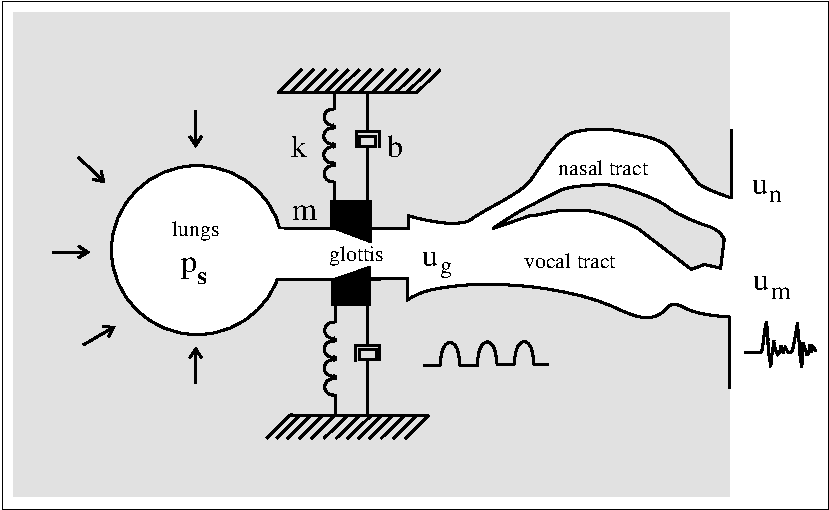
\includegraphics[width=80mm]{figure}}
\caption{{\it Schematic diagram of speech production.}}  
\label{spprod}
\end{figure}


\subsection{Hyperlinks}
For technical reasons, the proceedings editor will strip all active links from the papers during processing.
Hyperlinks can be included in your paper, if written in full, e.\thinspace{}g.\ "http://www.foo.com/index.html".
The link text must be all black.
Please make sure that they present no problems in printing to paper.


\subsection{Multimedia files}
The InterSpeech 2012 organizing committee offers the possibility to submit multimedia files.
These files are meant for audio-visual illustrations that cannot be conveyed in text, tables and graphs.
Just like you would when including graphics, make sure that you have sufficient author rights to the multimedia materials that you submit for publication.
The proceeding media will \emph{not} contain readers or players, so be sure to use widely accepted file formats and codecs, such as .mpg for video, .wav or .mp3 for audio,  and .png or .jpg for images.
The files you submit will be accessible from the abstract cards on the media and via a bookmark in the manuscript.
From within the manuscript, refer to a multimedia illustration by its filename.
Use short file names without blanks.


\subsection{Page numbering}
Final page numbers will be added later to the document electronically. 
{\em Don't make any footers or headers!}


\subsection{References}
The reference format is the standard IEEE one.
References should be numbered in order of appearance, 
for example here~\cite{ES1}, there~\cite{ES2}, and everywhere~\cite{ES3}.
Don't refer to citations as if they were parts of speech.


\subsection{Abstract}
The total length of the abstract is limited to 1000 characters.
The abstract included in your paper and the one you enter during web-based submission must be identical.
Avoid non-ASCII characters or symbols as they may not display correctly in the abstract book.


\subsection{Author affiliation}
Please list country names as part of the affiliation for each country.


\subsection{Submitted files}
Authors are requested to submit PDF files of their manuscripts.
You can use commercially available tools or for instance http://www.pdfforge.org/products/pdfcreator, or pdflatex.
The PDF file should comply with the following requirements:
(a) there must be no password protection on the PDF file at all;
(b) all fonts must be embedded; and
(c) the file must be text searchable (do CTRL-F and try to find a common word such as 'the').
The proceedings editors will contact authors of non-complying files to obtain a replacement.
In order not to endanger the preparation of the proceedings, papers for which a replacement is not provided timely will be withdrawn.


\section{Conclusions}
Authors must proof read their PDF file prior to submission to ensure it is correct.
Authors should not rely on proofreading their source file.
Please proofread the final PDF file before it is submitted.

\section{Acknowledgements}
The InterSpeech 2012 organizing committee would like to thank the organizing committee of InterSpeech 2008, 2009, 2010, 2011 for their help and for kindly providing the template files.

\eightpt
\bibliographystyle{IEEEtran}
\begin{thebibliography}{10}
\bibitem[1]{bahari} Bahari, M. H., et al., 
``Age Estimation from Telephone Speech using i-vectors'', 
Interspeech, 2012.

\bibitem[2]{dehak} Dehak, N., et al., 
``Front-End Factor Analysis for Speaker Verification'', 
IEEE Trans. Audio, Speech and Language Processing, 2011.

\bibitem[3]{garera} Garera, N. and Yarowsky D.,
``Modeling Latent Biographic Attributes in Conversational Genres'',
ACL/IJCNLP, 2009

\bibitem[4]{boulis} Boulis, B and Ostendorf, M.,
``A Quantitative Analysis of Lexical Differences Between Genders in Telephone Conversations'',
ACL, 2005

\end{thebibliography}
\end{document}
